% !TeX program = lualatex

% \documentclass[a4paper, 10pt]{article}
\documentclass{beamer}
\usetheme{metropolis}
\usepackage{cmbright}
\usepackage{tcolorbox}

% Encoding
\usepackage[T1]{fontenc}
\usepackage[utf8]{inputenc}
\usepackage[english]{babel}

% Mathematics
\usepackage{amsmath, amssymb, mathtools, amsthm}

% Bibliography (uncomment if needed)
\usepackage{csquotes}
\usepackage[backend=biber, sorting=none, style=nature]{biblatex}
\addbibresource{biblio.bib}

\newcommand{\dpdt}{\frac{\partial p}{\partial t}}
\newcommand{\dpdx}{\frac{\partial p}{\partial x}}
\newcommand{\ddpddx}{\frac{\partial^2 p}{\partial x^2}}

\title{}
\author{}

\begin{document}
  \begin{frame}{Single molecule perspective}\footnotesize
    \begin{figure}
      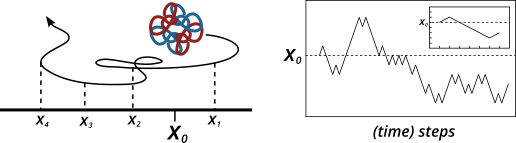
\includegraphics[width=\textwidth]{general.png}
    \end{figure}
    At every time step (the length of which is non trivial \cite{Verzelli,
    Gardiner1986HandbookOS}), the molecule can make a step $\eta$
    %
    \begin{equation*}
      \eta = \left\{ \begin{aligned}
        &\Delta x, &&\text{with probability} &&q\\
        &-\Delta x, &&\text{with probability} &&(1-q)\\
      \end{aligned}\right.
    \end{equation*}

    Let $X(t) \in \mathbb{R}$ be the position of the molecule after $N$ time
    steps ($t = N \, \Delta t$), we are interested in characterizing $\mathbf{p(x,N)}$, the
    \textbf{probability of the molecule being at position $\mathbf{x}$ after
    a time interval $\mathbf{t}$}.
  \end{frame}
  \begin{frame}{Fokker-Planck approach}\footnotesize
    The molecule can reach position x in one step only from $x+\Delta x$ or $x-
    \Delta x$.
    This allows us to write the recursive relation
    \begin{equation*}
      p(x, t + \Delta t) = q \, p(x-\Delta x, t) + (1-q) \, p(x+\Delta x, t)
    \end{equation*}
    If we expand to the first order in time and second in space, we obtain
    \begin{equation*}
      p + \Delta t \dpdt = 
      q \left(p - \Delta x \dpdx + \frac{\Delta x^2}{2} \ddpddx\right) + 
      (1-q) \left(p + \Delta x \dpdx + \frac{\Delta x^2}{2} \ddpddx\right)
    \end{equation*}
    which yields the \textbf{Fokker-Planck equation}
    \begin{center}
    \begin{tcolorbox}[width=6cm]
      \begin{equation*}
        \dpdt = D \, \ddpddx -v \dpdx
      \end{equation*}
    \end{tcolorbox}
    \end{center}
    with
    \begin{equation*}
      D = \frac{\Delta x^2}{2 \Delta t}, \qquad v = \frac{(2q - 1) L}{\Delta t}
    \end{equation*}
      

  \end{frame}  

  \printbibliography

\end{document}





